\section{Pipeline}
Di seguito, in figura \ref{fig:pipeline}, è presentata la pipeline del progetto, che illustra i vari passaggi e le fasi di elaborazione dei dati.

\begin{figure}[H]
    \centering
    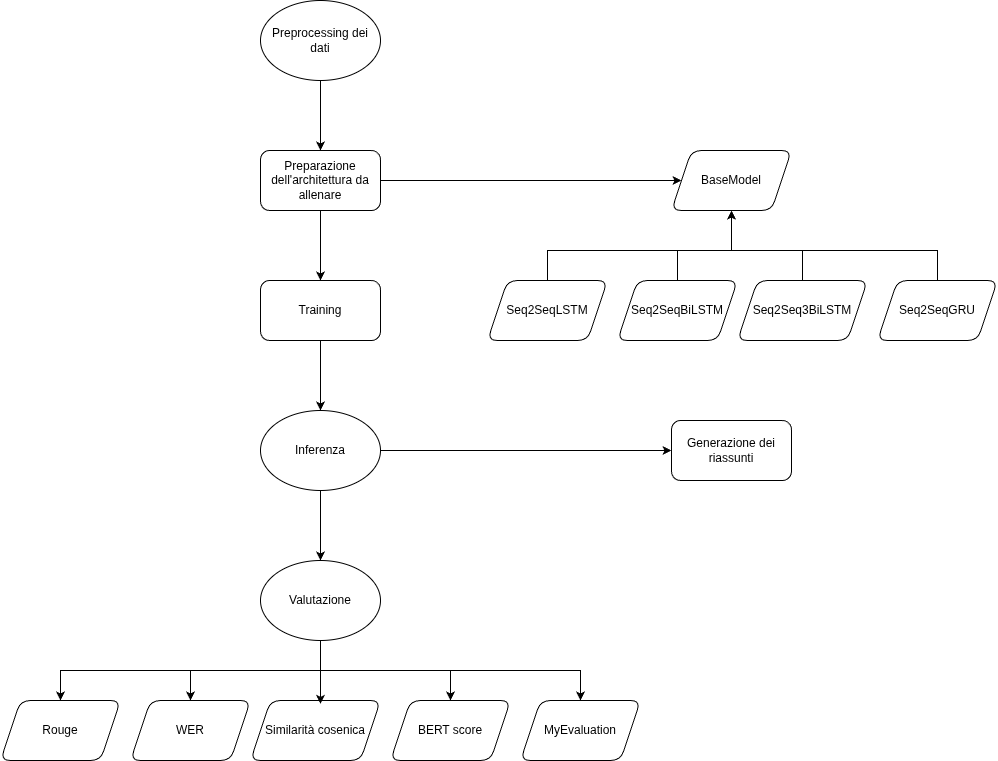
\includegraphics[width=1\textwidth]{media/pipeline.png}
    \caption{Pipeline del progetto}
    \label{fig:pipeline}
\end{figure}

La pipeline è suddivisa in tre fasi principali:
\begin{enumerate}
    \item \textbf{Preprocessing}: in questa fase vengono eseguite le operazioni di pulizia e preparazione dei dati, come la rimozione di stopwords, la tokenizzazione e la normalizzazione del testo.
    \item \textbf{Training}: in questa fase viene addestrato il modello di summarization utilizzando i dati preprocessati. Viene effettuata una suddivisione tra training set e validation set.
    \item \textbf{Evaluation}: in questa fase vengono valutati i riassunti generati dal modello utilizzando diverse metriche, come ROUGE, BERTScore e la metrica personalizzata \texttt{myevaluation}.
\end{enumerate}
Nelle sezioni successive, verranno approfonditi i dettagli di ciascuna fase della pipeline.